\subsection{Epiciklusi}
\label{sec:Epicycles}

Re\v{c} \emph{epiciklus}, u prevodu sa gr\v{c}kog, zna\v{c}i \emph{na krugu}, tj. \emph{krug na krugu}. Formalno, to je geometrijski model kori\v{s}\'c{}en da objasni varijacije u brzini i smeru kretanja Sunca, Meseca i ostalih planeta. Takav model je od gr\v{c}kih astronoma preuzeo i unapredio Ptolomej \footnote{Ptolomejev model je, kao i ostali modeli pre njega, pretpostavljao da je Zemlja u centru svemira. Medjutim, uprkos o\v{c}ito pogre\v{s}noj pretpostavci, njegov model je prvi precizno objasnio kretanje svemirskih tela}. Po Ptolomeju \cite{PtolemaicModel}, svaka planeta se kre\'c{}e po manjoj kru\v{z}noj putanji, zvanoj \emph{epiciklus}, dok se ta putanja kre\'c{}e po ve\'c{}oj kru\v{z}noj putanji, zvanoj \emph{deterent} (videti sliku \ref{img:PtolemaicModel}). 

\begin{figure}
    \centering
    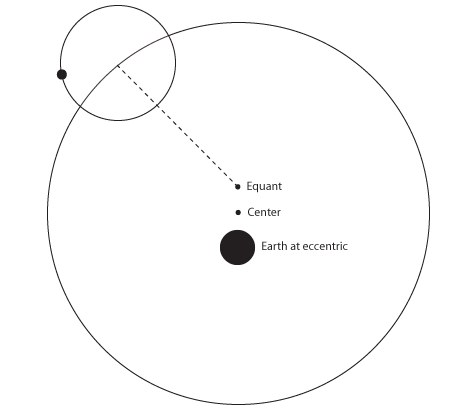
\includegraphics[scale=0.5]{images/ptolomaic_model.PNG}
    \caption{Ptolomejev model kretanja svemirskih tela.}
    \label{img:PtolemaicModel}
\end{figure}

Epicikluse mo\v{z}emo zakomplikovati rekurzivnim dodavanjem drugih epiciklusa. Dodati krugovi ne moraju (i \v{c}esto u primenama nisu) istih dimenzija. Postoje tvrdnje da je Ptolomejev model imao u opisima kretanja nekih planeta i do 80 epiciklusa, u poredjenju sa Kopernikovim sistemom, koji je imao do 34 epiciklusa \footnote{Nikola Kopernik je za cilj imao da smanji kompleksnost Ptolomejevog modela, \v{s}to je i uspeo u svom heliocentri\v{c}nom sistemu.}. Pokazano je da se bilo kakva putanja - bilo periodi\v{c}na ili ne, zatvorena ili otvorena - mo\v{z}e proizvoljno dobro aproksimirati \emph{slaganjem} dovoljnog mnogo epiciklusa odgovaraju\'c{}ih dimenzija (videti sliku \ref{img:pi}). U literaturi se takodje \v{c}esto za orbitu koju pravi poslednji krug koristi termin \emph{epiciklus}.

\begin{figure}
    \centering
    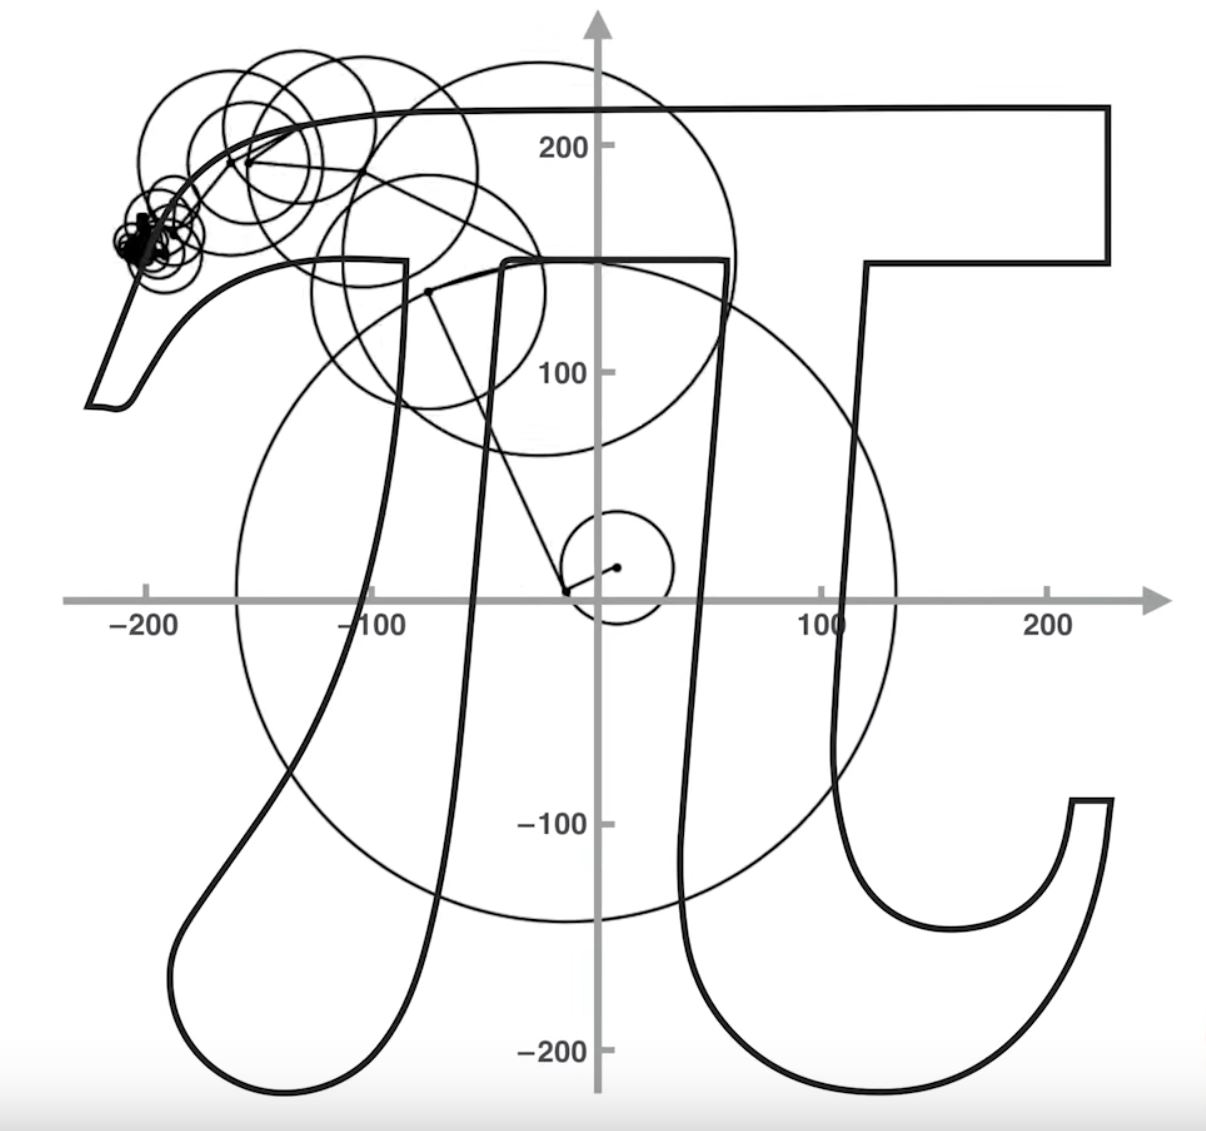
\includegraphics[scale=0.2]{images/pi.jpg}
    \caption{Demonstracija pra\'c{}enja orbite simbola $\pi$ pomo\'c{}u epiciklusa.}
    \label{img:pi}
\end{figure}

Epiciklusi se, naravno, mogu predstaviti potpuno formalno matemati\v{c}kim formulama. Deferent mo\v{z}emo predstaviti kao kompleksan broj
$$z_0 = a_0e^ik_0t,$$
gde su $a_0$ i $k_0$ konstante, $i$ imaginarna jedinica, a $t$ vreme. Deferent je stoga centriran u koordinatnom po\v{c}etku kompleksne ravni, sa polupre\v{c}nikom $a_0$ i ugaonom brzinom $k_0$ sa periodom $T$:
$$k_0 = \frac{2\pi}{T}.$$ 
Ukoliko je $z_1$ epiciklus, onda zbir deferenta i epiciklusa predstavlja periodi\v{c}nu funkciju \footnote{Zapravo, ovakve funkcije se nazivaju \emph{skoro periodi\v{c}ne funkcije} - zainteresovani \v{c}italac mo\v{z}e pro\v{c}itati vi\v{s}e u \cite{AlmostPeriodicFunctions}. Ova funkcija je periodi\v{c}na samo kada je udeo konstanti $k_j$ racionalan.}
$$z_2 = z_0 + z_1 = a_0e^ik_0t + a_1e^ik_1t.$$
Generalizovanjem dobijamo op\v{s}ti \v{c}lan:
$$z_n = \sum_{j=0}^{n}{a_je^ik_jt}$$

Postavlja se pitanje: \textit{\v{S}ta je zapravo putanja koju najmanji epiciklus pravi, i gde se ona krije u ovoj formuli}? Problem pronala\v{z}enja \emph{orbite} najmanjeg epiciklusa se sastoji u pronala\v{z}enju vrednosti koeficijenata $a_j$ kako bi se reprezentovao vremenski zavisan put u kompleksnoj ravni. Vi\v{s}e o tome u poglavljima koja slede.